% FNO architecture diagram (after Li et al. 2021, Fig. 2)
% Build:  cd Figures/src && pdflatex fno_architecture.tex && mv fno_architecture.pdf ..
\documentclass[tikz,border=4pt]{standalone}
\usepackage[T1]{fontenc}
\usepackage{lmodern}
\usepackage{amsmath,amssymb,bm}
\usepackage[dvipsnames]{xcolor}
\usetikzlibrary{arrows.meta,positioning,calc,fit,backgrounds}

% ---- palette ---------------------------------------------------------
\colorlet{lift}{Gray!18}
\colorlet{fourier}{NavyBlue!14}
\colorlet{fourierline}{NavyBlue!75!black}
\colorlet{local}{BurntOrange!18}
\colorlet{localline}{BurntOrange!85!black}
\colorlet{layer}{NavyBlue!7}

\begin{document}
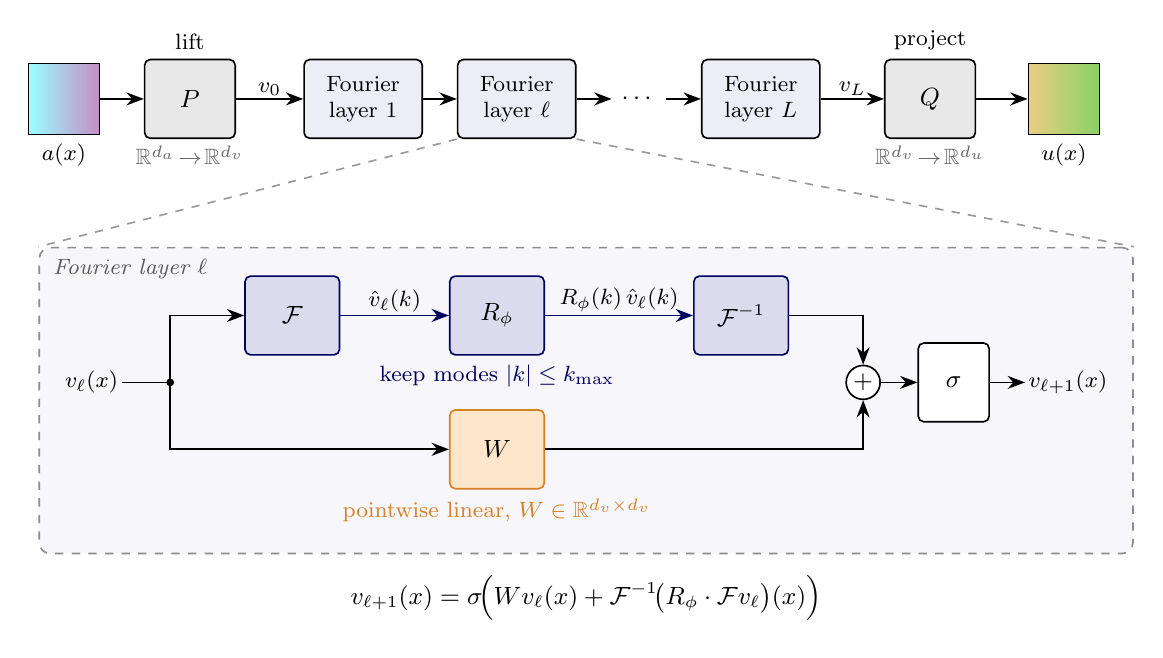
\begin{tikzpicture}[
    font=\small,
    >={Stealth[length=2.2mm]},
    every path/.style={line width=0.6pt},
    blk/.style={draw, rounded corners=2pt, minimum height=1.0cm,
                minimum width=1.15cm, align=center},
    lp/.style={blk, fill=lift},
    fl/.style={blk, fill=layer, minimum width=1.5cm, font=\footnotesize},
    sp/.style={blk, fill=fourier, draw=fourierline, minimum width=1.2cm},
    lo/.style={blk, fill=local, draw=localline, minimum width=1.2cm},
    field/.style={draw, minimum size=0.9cm, inner sep=0pt},
    lab/.style={font=\footnotesize, inner sep=1pt},
  ]

  % =================== top row: full network =========================
  \node[field, left color=Cyan!40, right color=Purple!45] (a) at (0,0) {};
  \node[lab, below=2pt of a] {$a(x)$};

  \node[lp] (P) at (1.6,0) {$P$};
  \node[lab, above=2pt of P] {lift};

  \node[fl] (L1) at (3.8,0) {Fourier\\layer $1$};
  \node[fl] (L2) at (5.75,0) {Fourier\\layer $\ell$};
  \node      (dots) at (7.3,0) {$\cdots$};
  \node[fl] (LL) at (8.85,0) {Fourier\\layer $L$};

  \node[lp] (Q) at (11.0,0) {$Q$};
  \node[lab, above=2pt of Q] {project};

  \node[field, left color=Goldenrod!55, right color=OliveGreen!45] (u) at (12.7,0) {};
  \node[lab, below=2pt of u] {$u(x)$};

  \draw[->] (a) -- (P);
  \draw[->] (P) -- node[lab, above] {$v_0$} (L1);
  \draw[->] (L1) -- (L2);
  \draw[->] (L2) -- (dots);
  \draw[->] (dots) -- (LL);
  \draw[->] (LL) -- node[lab, above] {$v_L$} (Q);
  \draw[->] (Q) -- (u);

  \node[lab, below=1pt of P, text=black!60] {$\mathbb{R}^{d_a}\!\to\!\mathbb{R}^{d_v}$};
  \node[lab, below=1pt of Q, text=black!60] {$\mathbb{R}^{d_v}\!\to\!\mathbb{R}^{d_u}$};

  % =================== bottom panel: one Fourier layer ===============
  \def\yU{-2.75}   % spectral path
  \def\yD{-4.45}   % local path
  \def\yM{-3.6}    % mid line

  \node[lab] (vin) at (0.35,\yM) {$v_\ell(x)$};
  \coordinate (split) at (1.35,\yM);

  \node[sp] (F)    at (2.9,\yU)  {$\mathcal{F}$};
  \node[sp] (R)    at (5.5,\yU) {$R_\phi$};
  \node[sp] (Fi)   at (8.6,\yU)  {$\mathcal{F}^{-1}$};
  \node[lo] (W)    at (5.5,\yD) {$W$};

  \node[draw, circle, inner sep=1pt, fill=white] (sum) at (10.15,\yM) {$+$};
  \node[blk, fill=white, minimum width=0.9cm] (sig) at (11.3,\yM) {$\sigma$};
  \node[lab] (vout) at (12.75,\yM) {$v_{\ell+1}(x)$};

  % wires
  \draw (vin) -- (split);
  \fill (split) circle (1.4pt);
  \draw[->] (split) |- (F);
  \draw[->] (split) |- (W);
  \draw[->, draw=fourierline] (F) -- node[lab, above] {$\hat v_\ell(k)$} (R);
  \draw[->, draw=fourierline] (R) -- node[lab, above] {$R_\phi(k)\,\hat v_\ell(k)$} (Fi);
  \draw[->] (Fi) -| (sum);
  \draw[->] (W) -| (sum);
  \draw[->] (sum) -- (sig);
  \draw[->] (sig) -- (vout);

  % path annotations
  \node[lab, below=2pt of R, text=fourierline] (Rnote)
       {keep modes $|k|\le k_{\max}$};
  \node[lab, below=2pt of W, text=localline] (Wnote)
       {pointwise linear, $W\in\mathbb{R}^{d_v\times d_v}$};

  % panel frame + title
  \begin{scope}[on background layer]
    \node[draw=black!45, dashed, rounded corners=4pt, fill=layer!50,
          inner xsep=8pt, inner ysep=10pt,
          fit=(vin) (F) (Fi) (W) (Wnote) (vout) (sum)] (panel) {};
  \end{scope}
  \node[lab, anchor=north west, font=\footnotesize\itshape, text=black!65]
       at ($(panel.north west)+(4pt,-3pt)$) {Fourier layer $\ell$};

  % zoom lines from layer ell to panel
  \draw[black!40, dashed] (L2.south west) -- (panel.north west);
  \draw[black!40, dashed] (L2.south east) -- (panel.north east);

  % equation under panel
  \node[below=4pt of panel, font=\small]
       {$v_{\ell+1}(x)=\sigma\!\Big(W v_\ell(x)
         + \mathcal{F}^{-1}\!\big(R_\phi\cdot\mathcal{F}v_\ell\big)(x)\Big)$};
\end{tikzpicture}
\end{document}
